
% ----------------------------------------------------------------------
%                   Latex File for Eamon O'Gorman's PhD (2013)
% ----------------------------------------------------------------------

%Latext thesis template from Harish Bhanderi's PhD/MPhil template, then Uni Cambridge
% http://www-h.eng.cam.ac.uk/help/tpl/textprocessing/ThesisStyle/

%: Style file for Latex
% Most style definitions are in the external file PhDthesisPSnPDF.
% In this template package, it can be found in ./Latex/Classes/
\documentclass[a4paper, oneside,12pt]{Latex/Classes/PhDthesisPSnPDF}

%Change "oneside" to "twoside" for final submission-grade thesis after viva/corrections

\usepackage{lineno}
\usepackage{amsbsy}
\usepackage{xspace}
\usepackage{wtmmPkg}
\usepackage{natbib}
\usepackage{multirow}
\usepackage{paralist}
\usepackage{titlesec}
\usepackage{lscape}
\usepackage{quotchap}
\usepackage{epstopdf}
\usepackage{fancyhdr}
\usepackage{graphicx}
\usepackage{amsmath}
\usepackage{float}
\usepackage{afterpage}

%Added by SM 13 Sep 2011 to get backref to read ''Cited on page''
   \usepackage{Latex/StyleFiles/backrefx}
       \renewcommand{\backrefpagesname}{Cited on page~}
       \renewcommand{\backrefpagesnames}{Cited on pages~}

\newcommand{\BibTeX}{\textsc{Bib}\TeX}
\newcommand{\etal}{{\it et al.}}

% Definitions for equations
\newcommand{\arcsec}{^{\prime\prime}}
%\def\ion#1#2{#1$\;${\small\rm\@Roman{#2}}\relax}
\DeclareRobustCommand{\ion}[2]{%
\relax\ifmmode
\ifx\testbx\f@series
{\mathbf{#1\,\mathsc{#2}}}\else
{\mathrm{#1\,\mathsc{#2}}}\fi
\else\textup{#1\,{\mdseries\textsc{#2}}}%
\fi}

\newcommand{\subion}{ {_{ion}} }
\newcommand{\sube}{ {_{e}} }
\newcommand{\subj}{ {_{j}} }
\newcommand{\subi}{ {_{i}} }
\newcommand{\ji}{ {_{j,i}} }
\newcommand{\rt}{ {$R(T)$} }
\newcommand{\rlam}{ {$R(\lambda)$} }
\newcommand{\rsun}{R$_{\odot}$}
\newcommand{\rmd}{ {\ \mathrm d} }
\renewcommand{\vec}[1]{ {\mathbf #1} }
\newcommand{\uvec}[1]{ \hat{\mathbf #1} }
\newcommand{\pder}[2]{ \f{\partial #1}{\partial #2} }
\newcommand{\grad}{ {\bf \nabla } }
\newcommand{\curl}{ {\bf \nabla} \times}
\newcommand{\vol}{ {\mathcal V} }
\newcommand{\bndry}{ {\mathcal S} }
\newcommand{\dv}{~{\mathrm d}^3 x}
\newcommand{\da}{~{\mathrm d}^2 x}
\newcommand{\dl}{~{\mathrm d} l}
\newcommand{\dt}{~{\mathrm d}t}
\newcommand{\intv}{\int_{\vol}^{}}
\newcommand{\inta}{\int_{\bndry}^{}}
\newcommand{\avec}{ \vec A}
\newcommand{\ap}{ \vec A_p}
\newcommand{\bb}{ \vec B}
\newcommand{\jj}{ \vec j}
\newcommand{\rr}{ \vec r}
\newcommand{\xx}{ \vec x}

% Definitions for the journal names
\newcommand{\adv}{    {\it Advances in Space Research}}
\newcommand{\annG}{   {\it Annales Geophysicae}}
\newcommand{\aap}{    {\it Astronomy \& Astrophysics}}
\newcommand{\aaps}{   {\it Astronomy \& Astrophysics Supplemental}}
\newcommand{\aapr}{   {\it Astronomy \& Astrophysics Review}}
\newcommand{\ag}{     {\it Ann. Geophys.}}
\newcommand{\aj}{     {\it Astronomical Journal}}
\newcommand{\apj}{    {\it Astrophysical Journal}}
\newcommand{\apjs}{    {\it Astrophysical Journal Supplemental Series}}
\newcommand{\apjl}{   {\it Astrophysical Journal Letters}}
\newcommand{\apss}{   {\it Astrophysics \& Space Science}}
\newcommand{\cjaa}{   {\it Chinese Journal Astronomy \& Astrophysics}}
\newcommand{\gafd}{   {\it Geophysical and Astrophysical Fluid Dynamics}}
\newcommand{\grl}{    {\it Geophysical Research Letters}}
\newcommand{\ijga}{   {\it International Journal of Geomagnetism and Aeronomy}}
\newcommand{\jastp}{  {\it Journal of Atmospheric and Solar-Terrestrial Physics}}
\newcommand{\jgr}{    {\it Journal of Geophysical Research}}
\newcommand{\mnras}{  {\it Monthly Notices of the Royal Astronomical Society}}
\newcommand{\nat}{    {\it Nature}}
\newcommand{\pasp}{   {\it Publications of the Astronomical Society of the Pacific}}
\newcommand{\pasj}{   {\it Publications of the Astronomical Society of Japan}}
\newcommand{\pra}{    {\it Physical Review A}}
\newcommand{\pre}{    {\it Physical Review E}}
\newcommand{\solphys}{{\it Solar Physics}}
\newcommand{\sovast}{ {\it Soviet Astronomy}}
\newcommand{\ssr}{    {\it Space Science Reviews}}
\newcommand{\araa}{  {\it Annual Review of Astronomy \& Astrophysics}}
\newcommand{\memsai}{ {\it Memorie della Societa Astronomia Italiana}}

%: Macro file for Latex
% Macros help you summarise frequently repeated Latex commands.
% Here, they are placed in an external file /Latex/Macros/MacroFile1.tex
% An macro that you may use frequently is the figuremacro (see introduction.tex)
% This file contains macros that can be called up from connected TeX files
% It helps to summarise repeated code, e.g. figure insertion (see below).

% insert a centered figure with caption and description
% parameters 1:filename, 2:title, 3:description and label
\newcommand{\figuremacro}[3]{
	\begin{figure}[htbp]
		\centering
		\includegraphics[width=1\textwidth]{#1}
		\caption[#2]{\textbf{#2} - #3}
		\label{#1}
	\end{figure}
}

% insert a centered figure with caption and description AND WIDTH
% parameters 1:filename, 2:title, 3:description and label, 4: textwidth
% textwidth 1 means as text, 0.5 means half the width of the text
\newcommand{\figuremacroW}[4]{
	\begin{figure}[htbp]
		\centering
		\includegraphics[width=#4\textwidth]{#1}
		\caption[#2]{\textbf{#2} - #3}
		\label{#1}
	\end{figure}
}

% inserts a figure with wrapped around text; only suitable for NARROW figs
% o is for outside on a double paged document; others: l, r, i(inside)
% text and figure will each be half of the document width
% note: long captions often crash with adjacent content; take care
% in general: above 2 macro produce more reliable layout
\newcommand{\figuremacroN}[3]{
	\begin{wrapfigure}{o}{0.5\textwidth}
		\centering
		\includegraphics[width=0.48\textwidth]{#1}
		\caption[#2]{{\small\textbf{#2} - #3}}
		\label{#1}
	\end{wrapfigure}
}

% predefined commands by Harish
\newcommand{\PdfPsText}[2]{
  \ifpdf
     #1
  \else
     #2
  \fi
}

\newcommand{\IncludeGraphicsH}[3]{
  \PdfPsText{\includegraphics[height=#2]{#1}}{\includegraphics[bb = #3, height=#2]{#1}}
}

\newcommand{\IncludeGraphicsW}[3]{
  \PdfPsText{\includegraphics[width=#2]{#1}}{\includegraphics[bb = #3, width=#2]{#1}}
}

\newcommand{\InsertFig}[3]{
  \begin{figure}[!htbp]
    \begin{center}
      \leavevmode
      #1
      \caption{#2}
      \label{#3}
    \end{center}
  \end{figure}
}


%%% Local Variables: 
%%% mode: latex
%%% TeX-master: "~/Documents/LaTeX/CUEDThesisPSnPDF/thesis"
%%% End: 


%Change this if compiling at home/office
%\graphicspath{{/Users/josephroche/Work/log_of_learning/images/}}
\graphicspath{{images/}}


%: --------------------------------------------------------------
%:                  FRONT MATTER: dedications, abstract,..
% --------------------------------------------------------------

\usepackage{setspace}
\singlespacing

\begin{document}

\renewcommand\baselinestretch{1.2}
\baselineskip=18pt plus1pt

%: ----------------------- COVER PAGE ------------------------

\newcommand{\titlefont}{\bfseries \fontsize{22}{26.42pt}\selectfont}
\newcommand{\largetitlefont}{\bfseries \fontsize{29.88}{35.88pt}\selectfont}
\newcommand{\othertitlefont}{\fontsize{14.4}{17.28}\selectfont}
\newcommand{\authorfont}{\bfseries \fontsize{14.4}{17.28}\selectfont}
\newcommand{\informationfont}{\fontsize{10}{12}\selectfont}
\newcommand{\dedicationfont}{\slshape \fontsize{14.4}{17.28}\selectfont}

\newcommand{\thisyear}{\number\year}
\def\thismonth{\ifcase\month\or January\or February\or March\or
  April\or May\or June\or July\or August\or September\or October\or November\or December\fi}
\newcommand{\todaysdate}{\thismonth\space \thisyear}

\renewcommand{\baselinestretch}{1}
\newpage \thispagestyle{empty}
\vspace*{1.5cm}
\begin{flushright}


%TITLE

\Huge{\textbf{Radio Interferometric Studies of Cool Evolved Stellar Outflows}}

\end{flushright}

\vspace*{4cm}
\begin{flushright}
A dissertation submitted to the University of Dublin \\
for the degree of Doctor of Philosophy
\end{flushright}

\vspace*{\fill}
\begin{flushright}
{\authorfont Eamon O'Gorman} \\[1mm]
Supervisor: Dr. Graham M. Harper\\[.5mm]
Trinity College Dublin, September 2013\\[.5mm]
\rule{0.9\textwidth}{0.5mm}\\[4mm]

\begin{minipage}[b][15mm][t]{12.5cm}
\raggedleft \sc
School of Physics\\
University of Dublin\\
Trinity College\\
\end{minipage}
\hspace*{1mm}
\begin{minipage}[b][15mm][t]{1.15cm}

\includegraphics[height=16mm]{tcd_crest.eps}
\end{minipage}

 \end{flushright}

%: ----------------------- tie in front matter ------------------------


\frontmatter

%!TEX root = ../thesis.tex
%Adding the above line, with the name of your base .tex file (in this case "thesis.tex") will allow you to compile the whole thesis even when working inside one of the chapter tex files


\begin{declaration}      

I declare that this thesis has not been submitted as an exercise for a degree at this or
any other university and it is entirely my own work.

\vspace{10mm}

I agree to deposit this thesis in the University's open access institutional repository or
allow the library to do so on my behalf, subject to Irish Copyright Legislation and
Trinity College Library conditions of use and acknowledgement.

\vspace{30mm}

\textbf{Name:} Eoin Carley	

\vspace{15mm}

\textbf{Signature:}  ........................................		\textbf{Date:}  ..........................



\end{declaration}

\newpage
\thispagestyle{empty}
\mbox{}


% ----------------------------------------------------------------------


%!TEX root = ../thesis.tex
%Adding the above line, with the name of your base .tex file (in this case "thesis.tex") will allow you to compile the whole thesis even when working inside one of the chapter tex files

\begin{abstracts} 

Coronal mass ejections (CMEs) are large-scale eruptions of magnetized plasma from the low solar atmosphere into interplanetary space. With energies of up to $10^{25}$\,J, they are the most energetic eruptive phenomena in the solar system and are also the driver of plasma shocks from the corona into the heliosphere. Despite many years of study, the nature of the forces governing their eruption, and the kinematical behavior of the resulting shock, remain poorly understood. In this thesis I will present the first accurate calculation of the magnitude of the total force on a CME. I will also present previously unobserved plasma shock behavior that sheds new light into the kinematical nature of CME-driven shocks in the corona.

In the past, measurement of the forces governing the propagation of CMEs have been hindered by highly uncertain estimates of the total mass of the ejection. The primary source of uncertainty is the unknown position and geometry of the CME, leading to an erroneous treatment of the Thomson scattering equations which are used to estimate the mass. Geometrical uncertainty on the CMEs position and size has primarily been due to observations of the eruption from a single vantage point. However, with the launch of the {\it Solar Terrestrial Relations Observatory (STEREO)}, the two viewpoints can be exploited to derive the CMEs position and size, ultimately resulting in mass uncertainty that is both reliably quantified and much reduced. Using the {\it STEREO} spacecraft, a CME on the 12 December 2008 was found to have a mass of $3.4\pm1.0\times10^{12}$\,kg, meaning the mass uncertainty was less than 30\%. This is a substantial improvement on previous uncertainties which were well above 50\%, or entirely unquantifiable. The much better mass estimates can then be combined with kinematical results that are also more reliable and hence lead to the first reliable quantification of the total force acting on the CME. The dynamics are described by an early phase of strong acceleration, dominated by a force of peak magnitude of $3.4\pm2.2\times10^{14}$\,N at $\sim$3\,$R_{\odot}$. Using the magnetohydrodynamics (MHD) equation of motion, the relative sizes of the forces at each stage in the CME propagation are estimated, revealing the Lorentz force is the largest source of CME acceleration early in its propagation. Quantification of the Lorentz force magnitude from observations has never been achieved in the past.


The second part of this thesis will involve an investigation into the behaviour of radio-bright plasma shocks occurring in the corona. CMEs often erupt at speeds in excess of the local magnetosonic wave speeds in the corona. Traveling in excess of Alfv\'{e}n Mach 1, they often drive shocks which can have a variety of observational manifestations, such as type II and III radio bursts, coronal bright fronts (CBFs), white-light enhancements, and the eventual in-situ detection of solar energetic particles. Despite such a variety of shock phenomena being observed for decades, the unifying physical mechanism between these phenomena remains unknown. This thesis will provide an analysis that uses extreme ultraviolet, radio, and white-light imaging of a solar eruptive event on 22 September 2011 to determine the properties of a CME-driven shock in the corona. The results show that a plasma shock with an Alfv\'{e}n Mach number of $2.4^{+0.7}_{-0.8}$ was coincident with a coronal bright front and an intense decametric radio burst generated by electrons with kinetic energies of 2-46\,keV (0.1-0.4\,c). This work provides new observational evidence to show that the relationship between CMEs, CBFs, and type II and III radio bursts is a coronal plasma shock. 



\end{abstracts}

% ---------------------------------------------------------------------- 

%!TEX root = ../thesis.tex
%Adding the above line, with the name of your base .tex file (in this case "thesis.tex") will allow you to compile the whole thesis even when working inside one of the chapter tex files

\begin{dedication} 

\large{\emph{For my parents.}}



\end{dedication}

% ----------------------------------------------------------------------
%!TEX root = ../thesis.tex
%Adding the above line, with the name of your base .tex file (in this case "thesis.tex") will allow you to compile the whole thesis even when working inside one of the chapter tex files





\begin{acknowledgements}      

Some sincere acknowledgements...

\end{acknowledgements}


% ------------------------------------------------------------------------



%!TEX root = ../thesis.tex
%Adding the above line, with the name of your base .tex file (in this case "thesis.tex") will allow you to compile the whole thesis even when working inside one of the chapter tex files
\chapter{List of Publications}
\label{chapter:publications}


\begin{enumerate}

\item \textbf{Carley, E.~P.}, MacAteer, R.~T. J., \& Gallagher, P.~T.\\
``Coronal Mass Ejection Masses, Energies, and Force Estimates Using \emph{STEREO}'', \\
\emph{The Astrophysical Journal}, Volume 752, Issue 1, article id. 36, 8 pp. (2012).

\item Zucca, P., \textbf{Carley, E.~P.},  McCauley, J., Gallagher, P. T. ,Monstein, C., \& MacAteer, R.~T. J.,\\
``Observations of Low Frequency Solar Radio Bursts from the Rosse Solar-Terrestrial Observatory'', \\
\emph{Solar Physics}, Volume 280, Issue 2, pp.591-602. (2012).

\item \textbf{Carley, E.~P.}, Long, D.~M., Byrne P. J., Zucca, P., \& Gallagher, P.~T.\\
``Quasi-periodic Acceleration of Electrons by a Plasmoid Driven Shock in the Solar Atmosphere '', \\
\emph{Nature Physics}, in press 

\item Zucca, P., \textbf{Carley, E.~P.}, Bloomfield, S.~D., \& Gallagher, P.~T.\\
``Density and Alfv\'{e}n....'', \\
\emph{Some Journal}, Volume X, Issue Y, article id. (2013)

\item Bloomfield, S.~D., \textbf{Carley, E.~P.},\\
``A Comprehensive Overview of the 2011 June 7 Solar Storm'', \\
\emph{Astronomy \& Astrophysics}, Volume X, Issue Y, article id. (2013)


\end{enumerate}





%: ----------------------- contents ------------------------

\setcounter{secnumdepth}{3} % organisational level that receives a numbers
\setcounter{tocdepth}{3}    % print table of contents for level 3
\tableofcontents            % print the table of contents
% levels are: 0 - chapter, 1 - section, 2 - subsection, 3 - subsection


%: ----------------------- list of figures/tables ------------------------

\listoffigures	% print list of figures
\listoftables  % print list of tables


%: --------------------------------------------------------------
%:                  MAIN DOCUMENT SECTION
% --------------------------------------------------------------

\mainmatter

\pagestyle{fancy}
%!TEX root = ../thesis.tex
%Adding the above line, with the name of your base .tex file (in this case "thesis.tex") will allow you to compile the whole thesis even when working inside one of the chapter tex files
%: ----------------------- introduction file header -----------------------
\chapter{Introduction}
\label{chap:1}

The Sun has long been the focus of humanity's curiosity. Throughout history it has been the harbinger of new religions, philosophies, and sciences. It has changed our understanding of our place in the Universe and allowed us to push forward the frontiers of stellar astronomy. Although our understanding of the Sun is nowadays more advanced, the curiosity we hold for it has not changed since the very early humans.
Now, we understand the Sun is a star similar to any other in its class, currently going through a relatively unchanging 11 year cycle of activity that is extremely rich in physical complexity. The study of such complex phenomena has yielded immeasurable advances in many areas of physics such as spectroscopy, plasma physics, magnetohydrodynamics (MHD), particle physics, to name but a few. Although some of these sciences have grown over decades (or even centuries) they are still incomplete. I hope this theses, in some small way, will contribute to the continuing growth of these sciences and to the understanding of our nearest star.


%Here is the introduction of the thesis, complete with a few references  \citep{sagan1997demon, prothero2007evolution}.  Section \ref{sec:1} contains Equation \ref{eqn:1}, Section \ref{sec:2} has Figure \ref{fig:1} and Section \ref{sec:3} has Table \ref{tab:1}. Chapter \ref{chap:2} has pretty much nothing in it.

\section{The Sun}\label{sec:1}

The Sun is our nearest star, located $1.49\times10^6$\,km from Earth at the centre of our solar system. Located on the main sequence of the Hetzpring-Russel (HR) diagram, it has a spectral class of G2V, with a luminosity of $L_{\odot}=(3.84\pm 0.04)\times10^{26}$\,W, mass of $M_{\odot}=(1.989\pm0.0003)\times10^{30}$\,kg and radius of $R_{\odot}=(6.959\pm0.007)\times10^8$\,m \citep{foukal2004}. It was born approximately $4.6 \times 10^9$\,years ago when a giant molecular cloud underwent gravitational collapse and began hydrogen nuclear fusion at its centre (reference). The energy produced from this fusion resulted in enough pressure to counteract gravitational contraction and bring about a hydrostatic equilibrium, allowing the young star to reach a stability that is sustained today. It is estimated the Sun will maintain this stability for another 5 billion years, at which point, it will move off the main sequence and into a red giant phase. During this later part of its life, it will grow in size to 100 times its current radius and begin nuclear burning of heavier elements such as carbon and oxygen. Once carbon burning in the core has ceased it can no longer sustain nuclear fusion of heavier elements, resulting in a gravitational instability that will eventually lead to a stellar nova. This nova will result in the loss of the outer envelopes and ultimately the Sun's death, leaving behind a compact and dense white-dwarf.

Until such time, the Sun will remain on the main sequence in a regular state of hydrogen fusion in its core. The energy released during this process is the ultimate source of light and all energetic activity that we observe from Earth and beyond. Before we can understand how this energy manifests in the solar atmosphere as a variety of energetic phenomena, it is important to understand how the energy is generated and transported through its interior and finally released into its atmosphere and interplanetary space.

\subsection{Solar Interior}\label{sec:10}

The theoretical development on how the solar interior is structured and how it behaves has been through what is known as the \textquoteleft standard solar model' or SSM. The SSM is a grouping of theories that described how the Sun was formed, how it maintains its stability, how it generates energy, and how this energy is transported through its interior and released at the surface. Much of the major developments of this theory have been in the 20th century, due mainly to the pioneering experiments in solar neutrino physics and helioseismsology. Hence, the development of the SSM has mainly been through a refinement of the theory based on these observational fields. Although the SSM has increased in sophistication, its four main aspects remain the most general framework for describing the behavior of the solar interior.

The SSM firstly states that the Sun was born from the gravitational collapse of a primordial gas of hydrogen, helium, and traces of other heavy elements. Secondly, it maintains its structural stability via a hydrostatic equilibrium such that the gravitational force is balanced by a pressure gradient ($\grad{P}=-\rho g$) at each radial distance inside the star. The third main aspect of the SSM involves the source of the Sun's energy. Much of the early ideas proposed during the 19th century involved some form of chemical reaction or energy released during a slow gravitational contraction. However, during the first half of the 20th century the theory that the Sun is at least as old as the Earth began to come into focus. The idea of the Sun being more than 4.5 billion years old prompted the question of what energy source could sustain the Sun's luminosity for such a length of time. It was soon realised that thermonuclear fusion must be the source of such energy, and, as a result, it should be possible to observe the neutrino products of this fusion. Hence, starting in the 1950s a number of pioneering neutrino physics experiments were developed in an attempt to detect solar-generated neutrinos at Earth. These pioneering experiments, as well as there more sophisticated counterparts today, confirm much of the theories on solar core energy generation.

From the 1950s onwards there has been a confirmed detection of neutrinos generated in a hydrogen fusion process, namely the proton-proton or \textquoteleft pp'-chain, in the solar core. In this process, four protons are fused to form a helium nucleus. This can occur in a variety of ways, but at the Sun's core temperature of 15 MK, the dominant reaction is the pp 1 chain given by
\begin{equation}
^{1}_1\mathrm{H} + ^{1}_1\mathrm{H} \rightarrow ~^{2}_1\mathrm{H} + e^{+}  + \nu_e
\end{equation}
\begin{equation}
^{2}_1\mathrm{H} + ^{1}_1\mathrm{H} \rightarrow ~^{3}_2\mathrm{He} + \gamma
\end{equation}
\begin{equation}
^{3}_2\mathrm{He}+^{3}_2\mathrm{He} \rightarrow ~^{4}_2\mathrm{He} + 2^{1}_1\mathrm{H}
\end{equation}
where $^{1}_1\mathrm{H}$ is a hydrogen nucelus, $^{2}_1\mathrm{H}$ is deuterium, $^{3}_2\mathrm{He}$ is tritium, $^{4}_2\mathrm{He}$ is helium, $e^{+}$ is a positron, $\nu_e$ is an electron neutrino, and $\gamma$ is a gamma ray photon. Reactions (1.1) and (1.2) must happen twice for (1.3) to occur. Taking this into account, the entire process may be summarised as 
\begin{equation}
4 ^{1}_1\mathrm{H}  \rightarrow ~^{4}_2\mathrm{He} + 2e^{+} + 2\nu_e + 2\gamma
\end{equation}
liberating $4.2\times10^{-12}$J of energy, with $\sim2.4$\% of the energy carried away by the neutrinos. This particular form of the pp-chain (pp 1) occurs in 86\% of the cases \citep{turk2011}. However, there are other reactions capable of producing He from H catagorized into pp II, pp III etc, which each involve production of $^7_4$Be and $^8_5$B. The initial neutrino detections at Earth were the result of the pp III reaction which involves the creation of $^8_5$B, followed by a decay to $^8_4$Be, a positron, and an electron neutrino \citep{davis1968}. These early detections and the results of more recent experiments such as the SuperKamiokande \citep{fukuda1998} show that the expected neutrino flux given by the standard solar model is smaller than the observed. This deficit in in neutrino flux observations became the famed \textquoteleft solar neutrino problem' during the 1970s. 
One of the proposed explanations for the process was via an oscillation of the neutrino amongst three sets of 'flavors' i.e., the neutrino can be either an electron $\nu_e$, muon $\nu_{\mu}$, or tau $\nu_{\tau}$ neutrino. With the original detectors only being able to detect the $\nu_e$, this would result in a flux deficit (non-detection of $\nu_{\mu}$ and $\nu_{\tau}$). This oscillation amongst three flavors was given the name the \textquoteleft MSW effect' after \citet{mikheev1986} and \citet{wolfenstein1978}, and later confirmed experimentally by the SuperKamionkande experiment.

The neutrino experiments together with the standard solar model SSM provide much of what we know about the solar energy generation and the solar core. They imply a temperature of $15.6\times10^6$K and density of $1.48\times10^5$\,kg\,m$^{-3}$ at solar centre, and also confirm the existence of a variety of pp reactions (pp 1 to pp IV), and some level of Carbon-Nitrogen-Oxygen (CNO) fusion process. These fusion processes occur over $0.0-0.25\,R_{\odot}$ (Figure~\ref{fig:solar_atmosphere}), which defines the solar core. Outside the core the temperature drops to a value such that fusion ceases. While thermonuclear fusion is the third aspect of the SSM involves the generation of solar energy, the fourth aspect involves exactly what happens to this energy once it is generated i.e., it describes an energy transport mechanism.


Beyond $0.25\,R_{\odot}$ the temperature drops to 8 MK, such that fusion stops but only free protons and electrons exist. In this environment, the photons continuously scatter off free particles, undergoing a random walk toward the surface over a distance of $0.25-0.7\,R_{\odot}$. This region is known as the radiative zone and has densities of $2\times10^4-2\times10^2$\,kg\,m$^{-3}$, resulting in a small photon mean free path (mfp) of $9.0\times10^{-4}$\,m. The photons proceed towards the solar surface over a very long time scale, taking on the order of $10^{5}$ years to traverse this region \citep{mitalas1992}. If radiative energy transport occurs, it will result in the following temperature gradient
\begin{equation}
\frac{dT}{dr} = -\frac{3}{16 \sigma}\frac{\kappa \rho}{T^3}F_{rad}
\end{equation}
where $\sigma$ is the Stefan-Boltzman constant, $\kappa$ is the mass extinction coefficient (opacity per unit mass), $\rho$ is mass density, $T$ is temperature, and $F_{rad}$ is the outward radiative flux. This implies that for a particular outward flux, if the opacity increases, a steeper temperature gradient is required to maintain such a flux. At $0.7\,R_{\odot}$ the temperature drops to 0.5\,MK allowing protons to capture electrons into a bound orbit. The existence of electrons in atomic orbit results in a dramatic increase in opacity of the plasma \citep{turk2011} and hence the temperature gradient increases. The increased temperature gradient required to sustain the energy flow may lead to the onset of a convective instability beyond $0.7\,R_{\odot}$ toward the solar surface. This instability will occur if the temperature gradient in the star is steeper than the adiabatic temperature gradient
\begin{equation}
\Bigg|\frac{dT}{dr}\Bigg|_{star} > \Bigg|\frac{dT}{dr}\Bigg|_{adiabatic}
\end{equation}
This is known as the Schwarzchild criterion, and it is fulfilled from $0.7-1\,R_{\odot}$ $-$a region known as the convection zone. The temperature and density drop as height increases and finally reaches T$\sim$$6000$\,K and mass densities of $\rho\sim1\times10^{-5}$\,kg\,m$^{-3}$. Although no complete theoretical treatment of convection exists, mixing length theory and hydrodynamical modeling are used to determine how convection occurs in the solar interior.

Much of what we know about the depth, temperature, and density of the core, radiative, and convection zones come from a fine-tuning of the standard solar model, such that the model reproduces observations from neutrino and helioseismology experiments. In fact helioseismology alone can indicate great detail of the internal structure of the Sun. It has revealed that both the core and radiative zone rotate as a rigid body, while the convective zone undergoes differential rotation (REFERENCE), in much the same way as the solar surface does. 
Hence the boundary between the radiative and convective zones mark a region where the internal dynamics of the Sun change dramatically. This boundary is known as the tachocline, and it is this region that is of much relevance to the generation and cyclic evolution of the Sun's magnetic field.


%The source of the Sun's energy is nuclear fusion in the solar core. Temperatures as high as $15\times10^{6}$\,K allow four protons to fuse and become a helium nucleus i.e., $4\,^{1}$H$\rightarrow ^{4}$He\,+\,2e$^{+}+2\nu+2\gamma$, in a process known as the proton-proton or pp-chain. Here e$^+$, $\nu$, and $\gamma$ are a positron, neutrino, and gamma ray photon, respectively, resulting from fusion processes in the pp-chain. The solar core extends to approximately $0.25\,R_{\odot}$ from solar center where hydrogen burning (fusion) stops. Beyond this point, energy transport is dominated by photons scattering off of free particles. The transport of energy via radiation continues up to $\sim0.8\,R_{\odot}$, at which point the temperature is low enough such that neutral atoms form and radiation can no longer propagate freely due to the high opacity. Between $\sim0.8-1\,R_{\odot}$ the temperature gradient is large enough for convection to become the dominant mechanism for the transport of energy to the solar surface


\begin{figure}[!h]
\begin{center}
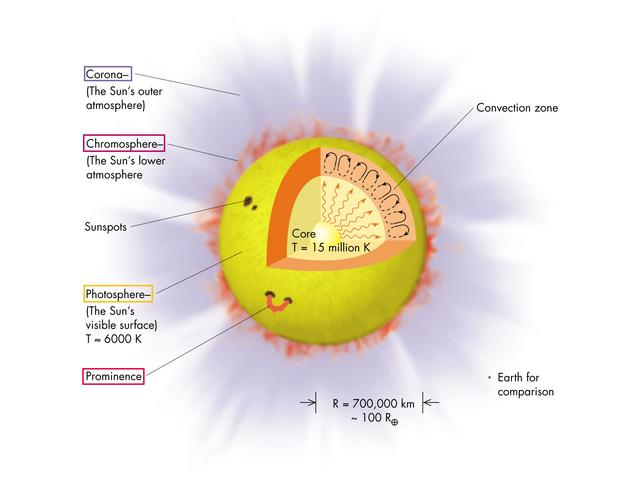
\includegraphics[trim = 0cm 0.5cm 0cm 0cm, width=1.0\textwidth]{images/solar_atmosphere}
\caption{The internal structure of the Sun, including the core, radiative zone, and convective zone.  Also shown is the structure of the its atmosphere, including the photosphere, chromosphere, and corona. The layers of the solar atmosphere are usually demarcated by temperature changes as height above the solar surface increases. The temperature ranges from $\sim$6000\,K in the photosphere to above 1\,MK in the corona.}
\label{fig:solar_atmosphere} 
\end{center}
\end{figure}



\subsection{Solar Dynamo and Magnetic Field}\label{sec:11}

\begin{itemize}
\item Cellular pattern in photosphere is very different to the convective structure in deeper layers.
\end{itemize}


\begin{figure}[!h]
\begin{center}
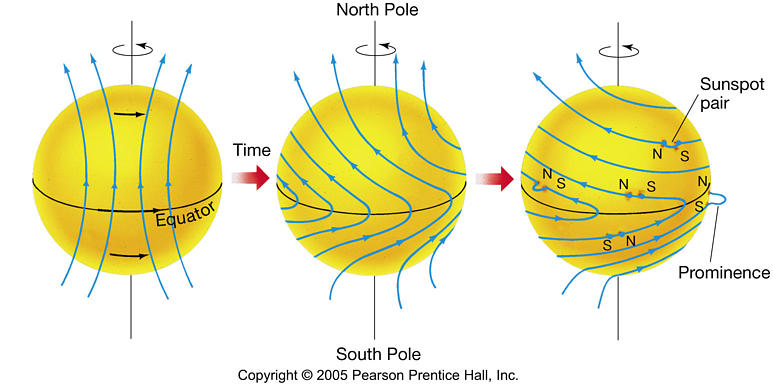
\includegraphics[]{images/Babcock}
\caption{Differential rotation and flux freezing result in the poloidal dipolar magnetic field, generated by dynamo action, to be dragged around in a toroidal direction, an action known as the omega effect. Buoyancy of the field lines results in them rising and twisting, known as the alpha effect, eventually surfacing to become bipolar fields that extend far into the corona.}
\label{fig:Babcock} 
\end{center}
\end{figure}

It is widely believed that the Sun's magnetic field is created by a dynamo action in a region between the radiative zone and the convection zone, known as the tachocline. Solar dynamo theory attempts to explain the observed 11 year magnetic activity cycle, where the the Sun's magnetic field starts as a poloidal dipolar structure and evolves to having a strong toroidal component, after which it returns to a poloidal field again. During these 11 years the Sun starts at minimum activity, reaches a maximum and returns to minimum again.

\citet{babcock1961} first explained this process by a mechanism involving differential rotation of the solar surface and interior. The equatorial rotation rate is faster than the rotation rate at higher latitudes. Because the magnetic field is frozen into the plasma, any flows in the solar interior will tend to drag the magnetic field along. By this effect, differential rotation tends to drag the field and wrap it around the Sun in a toroidal direction, this is known as the omega effect, see Figure~\ref{fig:Babcock}.

As the toroidal field builds up in the solar interior, sections of field lines build up in magnetic pressure resulting in a buoyancy of the field. The field slowly rises through the convection zone and eventually surfaces as a bipolar region that extends into the solar atmosphere. The presence of bipolar fields in the solar atmosphere and their slow build up over time to complex magnetic structures, known as active regions, ultimately leads to a variety of eruptive phenomena.



\subsection{Solar Atmosphere}\label{sec:12}

\subsubsection{Photosphere}\label{sec:121}

\begin{itemize}
\item Appearance, Granules, Sunspots.
\item Black Body Curve. Franhofer lines, H-alpha line, CaII H \& K, H$^{-}$ alines, Sodium D lines. 
\item Temperature, Density, Opacity.
\item Magnetic field strength
\end{itemize}

The most spectacular and energetic phenomena in our solar system have their origins in the solar atmosphere. This ever-changing and dynamic environment is a hotbed of activity giving rise to coronal mass ejections (CMEs), solar flares, and a host of plasma processes resulting in emission across the entire electromagnetic spectrum. To make sense of the phenomena we observe we must first have a basic understanding of solar atmospheric structure and the environment these processes take place in. Figure~\ref{fig:solar_atmosphere} is an illustration of the different layers of the solar interior, the solar surface and atmosphere. The visible surface of the Sun is known as the photosphere. It is demarcated where optical depth becomes unity for a wavelength of 5000\,\AA\ or $\tau_{5000}=1$. At such visible wavelengths, the electromagnetic spectrum is well represented by a blackbody of temperature T$\sim$6000\,K. .

\begin{itemize}
\item Eddington Barbier, $\tau=\mu$, limb darkening.
\item Effective temperature, $\tau=2/3$, $T=5800$\,K
\end{itemize}

During periods of increased activity there may also be the presence of sunspots in the photosphere. These are dark features on the solar surface, see Figure~\ref{fig:solar_atmosphere}, and are an indicator of concentrations of magnetic fields that are stronger than elsewhere in the quiet sun, as described above. 

Photospheric abundances have been measured using emission line diagnostics were it is found that helium is the most abundant at 10.89\footnote{Abundances quoted relative to hydrogen on a logarithmic scale, $12.0+log_{10}(A/A_H)$}, with the next most abundant elements being Carbon (8.58), Nitrogen (8.02), and Oxygen (8.8). All other elements have abundances that are 4 orders of magnitude or more less than hydrogen i.e., logarithmic abundances $\lesssim7$ \citep{phillips2008}.

\subsubsection{Chromosphere}\label{sec:122}

\begin{itemize}
\item Appearance, Supergranular Network, Bright Points, Spicules, Filaments, Plage etc.
\item Emission lines, H-alpha, CaII H \& K. 
\item Temperature, Density, Opacity.
\item Magnetic field strength.
\end{itemize}

At $\sim$500\,km above the $\tau_{5000}=1$ surface the temperature drops to a minimum of $\sim$4400\,K. Beyond this minimum the temperature begins to rise again, demarcating the beginning of the chromosphere. This layer of the atmosphere is generally accepted to extend to a height at which temperatures reach 20,000\,K, however temperatures as high as $\sim1\times10^5$\,K are sometimes attributed to chromospheric heights, hence it is observable at ultraviolet (UV) wavelengths as well as visible. 

\subsubsection{Corona}\label{sec:123}

\begin{itemize}
\item Appearance UV: Active regions, Coronal Loops, Holes.
\item Emission lines, Mg, Ca, Fe, C, O etc.
\item Appearance White-Light: Streamers, K, F, E corona
\item Appearance Radio: thermal bremsstrahlung, free-free emissivity/opacity.
\item Temperature, Density, Opacity, 'coronal heating problem'.
\end{itemize}


At a height of approximately 2,000\,km the temperature begins to rise sharply while the number density of neutral hydrogen and electrons fall by several orders of magnitude. This rapid increase in temperature in such a short spatial extent ($<$100\,km) is known as the transition region. It has a temperature on the order of $10^5$\,K and separates the relatively low temperature chromosphere and the high temperatures of $>1$\,MK in the corona. The reason for this rapid increase in temperature is still a hotly debated subject and a coronal heating mechanism remains largely unknown, this is known as the  \textquoteleft coronal heating problem'.


Element abundances in the corona show there is a similar composition to the photospheric abundances, with He, C, N, and O having the same ratios relative to H in the corona as that in the photosphere. The only difference is an enhancement in the abundance of low First Ionization Potential ($<10$\,eV) elements in the corona relative to the photosphere. For example, elements such as Na, Mg, Al, Si, Ca, Ni, and Fe can be up to three times more abundant in the corona \citep{feldman2003}. The reason for the enhancement of low FIP elements in the corona is still unknown, however several models have suggested ion-neutral separation in the chromosphere by diffusion across magnetic fields, followed by transport of these ions into the corona may be viable mechanism \citep{geiss1985}. 


\subsection{Solar Wind}\label{sec:13}

\begin{itemize}
\item Parker's solution
\item Parker Spiral
\item Fast solar wind, Alfv\'{e}n wave driver
\item Mass loss rates (later compare CME mass loss)
\end{itemize}



\section{Coronal Mass Ejections and Coronal Shocks}\label{sec:2}

\subsection{CMEs}\label{sec:20}

\begin{itemize}
\item Appearance, white-light Illing, Hundhausen, Vourlidas
\item Kinematics, velocity, acceleration
\item Dynamics, masses, energies, forces
\item Observations at other wavelengths, EUV, radio, SXR.
\end{itemize}

\subsection{CMEs and Shocks}\label{sec:21}

\begin{itemize}
\item Radio bursts, Type II, Type III
\item Radio imaging of shocks
\item Relationship to EUV waves, Moreton waves
\end{itemize}

\subsection{Open Questions}\label{sec:22}






	
\include{2/intro_to_radio}
\include{3/instrum_tar_obs}
\include{4/data_analysis}
\include{5/aori}
\include{6/aboo_atau}


% --------------------------------------------------------------
%:                  BACK MATTER: appendices, refs,..
% --------------------------------------------------------------
\appendix

%!TEX root = ../thesis.tex
%Adding the above line, with the name of your base .tex file (in this case "thesis.tex") will allow you to compile the whole thesis even when working inside one of the chapter tex files

\chapter{A Nice Appendix}
\label{app:1}

If we assume the herringbones are due to the shock drift acceleration process then the velocity upon a reflection from the shock is
\begin{equation}
v_{r,||} = 2v_{shock}\mathrm{sec}\,\theta_{Bn} - v_{i,||}
\end{equation}
where $v_{r,||}$ is the reflected parallel velocity of the particle, $v_{i,||}$ is the incident parallel velocity of the paticle, $v_{shock}$ is the shock velocity, and $\theta$ is the angle between upstream $B-$field and shock normal $n$. Taking the shock speed to be the speed of the 150\,MHz radio source, $550\times10^3$\,m\,s$^{-1}$, and $v_{i,||}$ to be the thermal speed of an electron 
\begin{equation} 
v_{thermal} = \sqrt{ \frac{3k_bT}{m_e} }
\end{equation}
At $1\times10^{6}$\,K, $v_{thermal} = v_{i,||} = 6.7\times10^6$\,m\,s$^{-1}$. Now, the herringbone electron speed 0.15\,c, this is the reflected speed $v_{r,||}$ in equation A1. Rearranging A1 we get
\begin{equation}
\theta_{Bn} = \mathrm{sec}^{-1}\bigg( \frac{1}{2}\frac{v_{r,||} +  v_{i,||} }{v_{shock}}\bigg)
\end{equation}
Substituting the above values we get $\theta_{Bn}=88^{\circ}$. Independent verification of a quasi-perpendicular shock orientation!



\section{Radio burst intensity}


\begin{equation}
\Phi_F \approx 72\sqrt{3}   \frac{\gamma_{L^{'}}}{\gamma_S}   \frac{v_e^3}{c^3}   \frac{v_b}{\Delta v_b}   \frac{e^{-u_c^2}}{u_c\sqrt{\pi}}  \zeta_F
\end{equation}
\begin{equation}
\Phi_H \approx \frac{18\sqrt{3}}{5\gamma_t}   \sqrt{\frac{m_i}{\gamma_t m_e}}  \frac{v_e^3 v_b^3}{c^5} \frac{v_b}{\Delta v_b}\zeta_H
\end{equation}
the expression involving $u_c$ represent an \textquoteleft escape factor' for the fundamental taking into account absorption and scattering of the radiation. $ \frac{\gamma_{L^{'}}}{\gamma_S} $ is the ratio of the damping rates of the product waves out of processes in equations~\ref{eqn:harm} and \ref{eqn:fund}. The $\zeta$ terms are the fractions of Langmuir waves that are kinematically able to contribute to the fundamental or harmonic emission, given by

\begin{equation}
\zeta_F  \approx \mathrm{exp} \bigg[  -\frac{4\gamma_t m_e}{45 m_i}    \bigg(\frac{v_b}{\Delta v_b}\bigg)^2   \bigg(  \frac{3}{2}  \sqrt{\frac{m_i}{\gamma_t m_e}} - \frac{v_b}{v_e}  \bigg)^2    \bigg]
\end{equation}

\begin{equation}
\zeta_H \approx \frac{c}{2v_b} \sqrt{\frac{\pi}{6}} \frac{\beta \Delta v_b}{v_b}
\Bigg[  \mathrm{erf}\Bigg(     \frac{ \frac{v_e\sqrt{3}}{c}  + \frac{2}{3} \sqrt{\frac{\gamma_t m_e}{m_i}}  }  {\frac{v_e}{v_b} \frac{\beta \Delta v_b}{v_b} \sqrt{2} }   \Bigg)     +   \mathrm{erf}\Bigg(     \frac{ \frac{v_e\sqrt{3}}{c}  - \frac{2}{3} \sqrt{\frac{\gamma_t m_e}{m_i}}  }  {\frac{v_e}{v_b} \frac{\beta \Delta v_b}{v_b} \sqrt{2} }   \Bigg)   \Bigg]
\end{equation}
where erf is the error function. 


\section{Band-splitting}
Using a ploytropic index of $\gamma=5/3$ (monatomic) means the shock compression can be no more than a factor of 4. Another extremely important fact arising from this is that magnetic compression can also be no greater than 4 i.e., from equation 4(b) $B_{2}/B_{1}=\chi$. $\chi<4$ has consequences for the shock drift acceleration mechanism and provides an upper limit to the particle energy gain

may also provide an upper limit to the level of band splitting in type II radio bursts (since this effect is thought to be related to the emission induced up/downstream of the shock). Although the maximum compression ration of 4 was derived from the roots of the quadratic for $\chi$ for the perpendicular shock, a similar analysis for the much more general oblique shock also leads to the same result. The density compression and tangential magnetic compression can be no more than a factor of $(\gamma+1)/(\gamma-1)$ for any MHD shock. 

%In either the perpendicular case or the general 2D oblique case a polynomial expression for the compression ratio (such as (6)) may be derived. The general oblique shock case requires extra terms in the polynomial such as $M_{A},\beta,\gamma,\theta_{Bn},\theta_{vn}$ ($\theta_{Bn}$ is the angle between shock normal and magnetic field, and $\theta_vn$ is the angle between shock normal and plasma flow). 
Polynomials such as (6) are extremely useful, and can lead to simple expressions for the Alfv\'{e}nic-Mach number in terms of $\chi$, in this case
\begin{equation}
M_{A}=\sqrt{\frac{\chi(\chi+5+5\beta)}{2(4-\chi)}} 
\end{equation}
for a perpendicular shock. If the shock speed and compression ratio are known, this equation provides a means of measuring the Alfv\'{e}n speed in the shock medium. 

This technique is exploited in the analysis of type II radio bursts. As the shock propagates into the corona it emits EM radiation at the local plasma frequency (1) (see section 4), and since the density drops as the shock travels into the heliosphere, so too does the frequency of emission. From frequency drift rate an estimate of shock speed is possible. If band splitting of the emission is present this is interpreted as emission from upstream and downstream of the shock, which provides a diagnostic of upstream/downstream densities via (1) and hence an estimate of $\chi$ \citep{vrsnak2002}. However, use of (8) in calculating Mach number and Alfv\'{e}n speed in the corona has some clear shortcomings such that it clearly ignores any dependency of the angle between magnetic field, velocity vector and shock normal i.e., (8) only applies to a purely perpendicular shock.

The general oblique shock case requires extra terms in the polynomial such as $\theta_{Bn}$ and $\theta_{vn}$ ($\theta_{Bn}$ is the angle between shock normal and magnetic field, and $\theta_{vn}$ is the angle between shock normal and plasma flow). For the oblique case the polynomial becomes
\begin{equation}
(A^2-\chi)^2\bigg[A^2 - \frac{2\chi S^2}{\chi+1-\gamma(\chi-1)}\bigg]\\
-\chi k^2A^2\bigg[\frac{2\chi - \gamma(\chi-1)}{\chi+1- \gamma(\chi-1)}A^2 -\chi\bigg]=0
\end{equation}
where $A=\frac{M_A\mathrm{cos}\theta_{vn}}{cos(\theta_{Bv}-\theta_{bn})}$,  $S=\frac{c_s}{v_A}$, $k=\mathrm{tan}(\theta_{vn}-\theta_{Bv})$ \footnote{$\theta_{Bv}$ is angle between magnetic field and velocity vector, it has a simple relationship with $\theta_{Bn}$} 
\citep{kabin2001}. Equation (6) is a quadratic of variable $\chi$, the more general equation (9) is a cubic equation for $\chi$, the roots of which give the compression for the oblique case. Since it is a function of $M_A$, $\theta_{vn}$, and $\theta_{bv}$, $\chi$ may have a range of values depending not only on Mach number but also shock orientation. Figure 2 illustrates the broad range in compressions of 0$<\chi<$3.5 across the shock depending on both flow and magnetic field orientation with respect to the shock normal, and in this case $M_A=2.5$. 
%\begin{figure}[h!]
%\includegraphics[scale=0.5, angle=270,trim =  3cm 0cm 4cm 0cm]{data/vary_thetaVn_thetaBn_mach2_5.pdf}
%\caption{Image and surface plot of compression ratio (from the solutions of (9)) as a function of $\theta_{vn}$ and $\theta_{Bn}$, with an Alfv\'{e}n Mach number of 2.5. The range of compressions is from 0 to 3.5 depending on the orientation of the magnetic field and velocity vectors with respect to the shock normal. Any discontinuities or sharp jumps are an indication of where the solutions to (9) are multi-valued.}
%\label{fig:vary_thetaVn_thetaBn_mach2_5}
%\end{figure}
This is a very general case, however, permitting any angle of orentation of $B$ and $v$. Since type II bursts are thought to be from shocks that are quasi perpendicular, this places restriction on the values for $\theta_{vn}$, and $\theta_{Bn}$, especially when the flow is considered to be head-on i.e. $\theta_{vn}=0^{\circ}$. Therefore in the quasi-perpendicular case their is a tighter constraint on the amount of compression across the shock. Further constraining the Mach number to a limited range of values puts quite a limiting range on the compression ratio, and hence a limiting range of band splitting of type II radio bursts since $f_{plasma}\approx9000\sqrt{n_e}$, hence
\begin{equation}
\delta_{bs} \equiv \frac{f_{upper}}{f_{lower}} \approx \sqrt{ \frac{ n_{e,d} }{ n_{e,u} } }=\sqrt{\chi}
\end{equation}
where $n_{e,d}$ and $n_{e,u}$ are downstream and upstream plasma number densities, and $\delta_{bs}$ is the ratio of upper to lower band frequencies, $f_{upper}$ and $f_{lower}$ respectively, in a split radio burst. Figure 3 shows the expected range in band splitting ($\delta_{bs}=\sqrt{\chi}$) for a type II given a range in Alfv\'{e}n Mach numbers $1<M_A< 4$, and quasi-perpendicular magnetic field orientations $45^{\circ}<\theta_{Bn}<90^{\circ}$. 
\begin{figure}[h!]
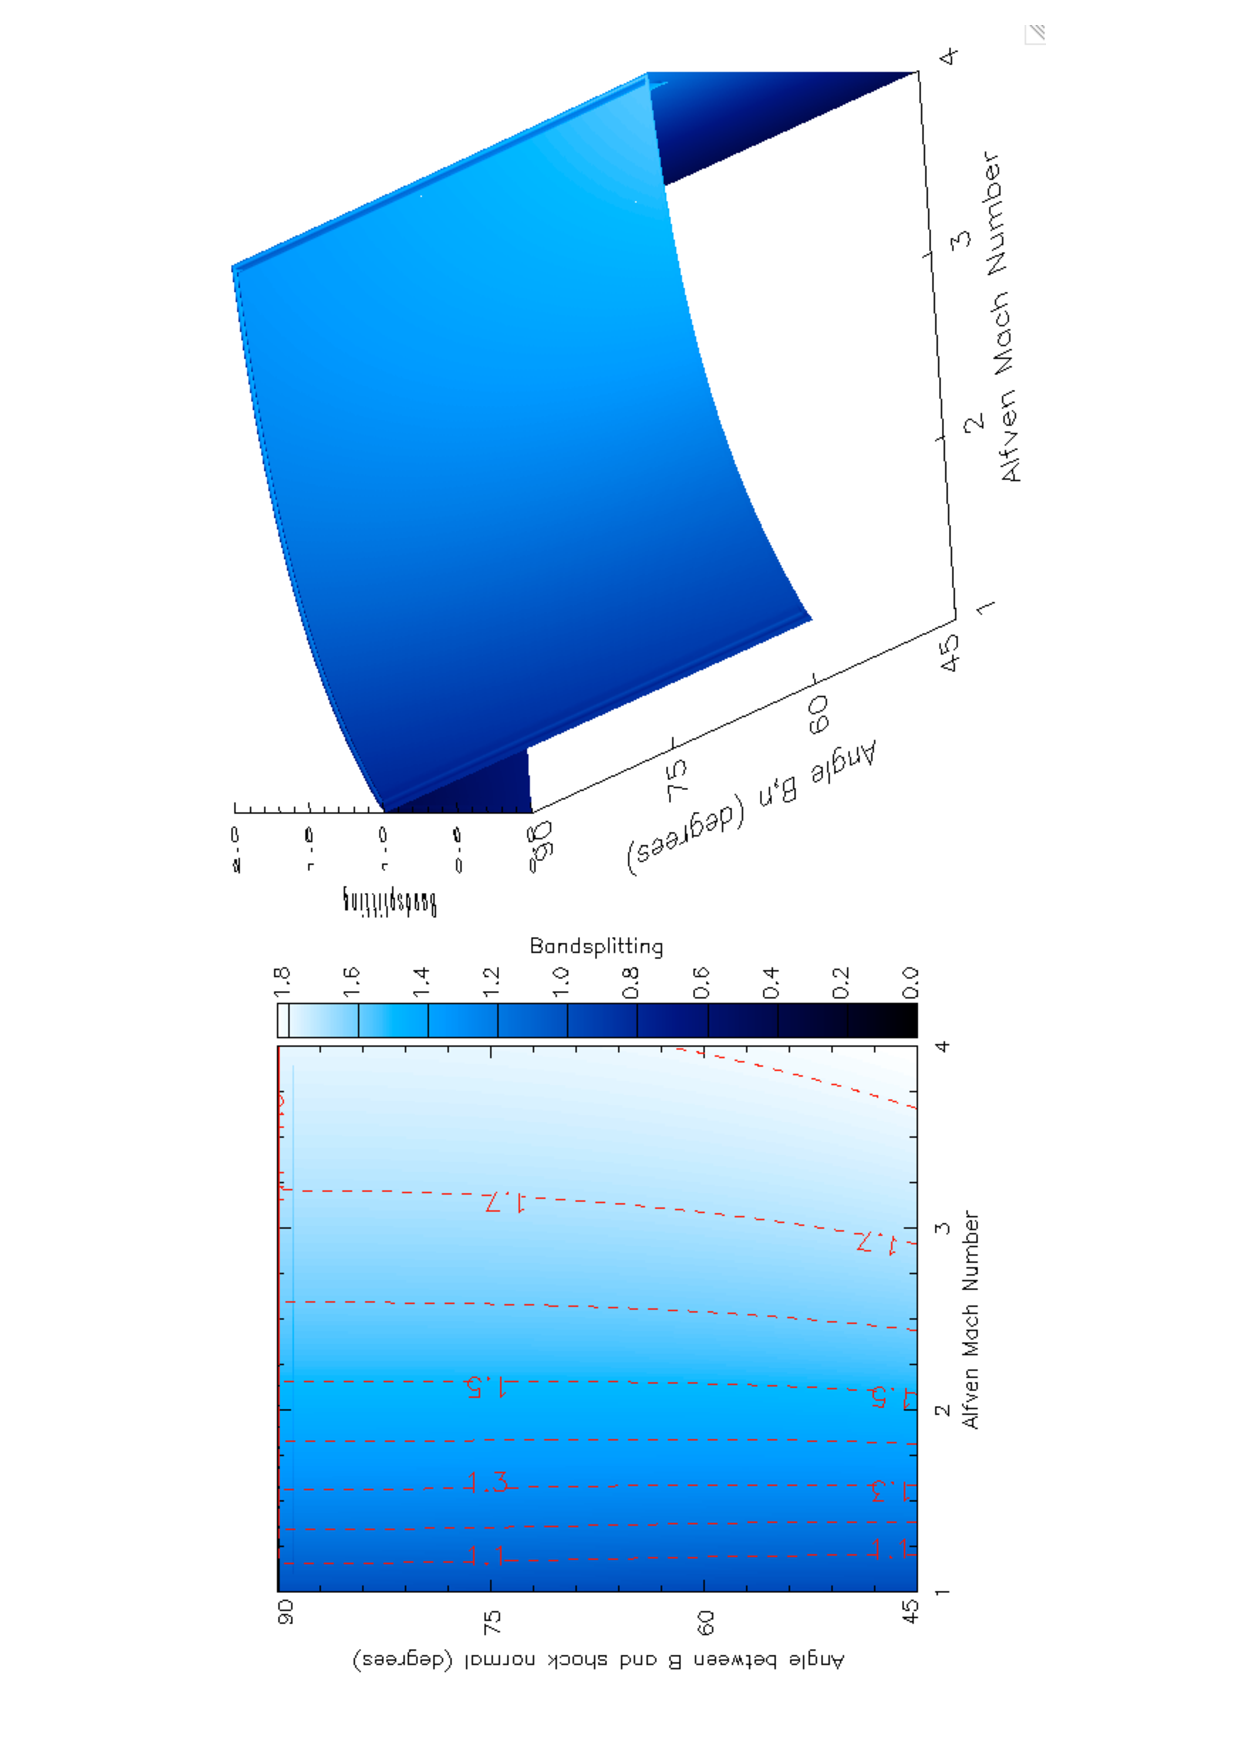
\includegraphics[scale=0.5, angle=270,trim =  3cm 0cm 4cm 0cm]{images/MHD_vary_mach&thetaBn.pdf}
\caption{Predicted band splitting ratio $\delta_{bs}$ as a function of Mach number and magnetic field orientation with respect to shock normal. Flow is anti-parallel to shock normal (head-on). Both image and surface are shown, left and right respectively. On the left, the red contours show specific values of of band-splitting. Note that for small mach numbers the level of band splitting is independent of magnetic field orientation. It is only at Mach numbers greater than $\sim$2.1 that the B-field orientation becomes important.}
\label{fig:MHD_vary_mach&thetaBn}
\end{figure}
This analysis shows that for a quasi-perpendicular shock the theoretically predicted range in type II band-spliting is $1<\delta_{bs}<1.8$. Such an upper limit to the level of band-splitting seems excessive and is probably due to a large upper limit to the Mach number being used to calculate the compression ratio. This is especially relevant in the low corona where Alfv\'{e}n speed can be quite large, making it difficult for a CME or blast wave to drive a shock at $M_A=4$. Also, given a typical band-splitting ratio of $\delta_{bs}=1.21\pm0.7$ at metric wavelengths \citep{vrsnak2004}, this would indicate typical Alfv\'{e}n-Mach number of $\sim\,1.5$ in the low corona. This seems reasonable, however Mach numbers of $\sim$3 are possible, and figure 3 would suggest a possible band-split ratio of $\delta_{bs}\sim1.7$ for such a Mach number. Such a level of band-splitting seems very unlikely, suggesting a quasi-perpendicular shock with a head on flow is a limiting case. More likely is a quasi-perpendicular shock with a flow orientation $\theta_{vn}\neq0$. For example if $\theta_{Bn}=90^{\circ}$ and $\theta_{vn}=45^{\circ}$ then band splitting can be $\delta_{bs}\sim\,1.5$ for $M_A$=3, which is under the upper limit of observed type II band-split ratios of $\sim\,1.58$. Allowing $\theta_{vn}\neq0$ can allow larger, more realistic Mach numbers to produce smaller and more realistic bandsplitting.


It is clear that the distribution in the level of band splitting in type II radio bursts depends not only on Mach number but the relative orientations of flow and magnetic field with respect to shock normal. A statistical analysis could possibly give an observationally predicted distribution in $\theta_{Bn}$ (provided $M_A$ is known) that would confirm the quasi-perpendicularlity of type II-generating shocks.




%: ----------------------- bibliography ------------------------

\begin{footnotesize} 
\bibliographystyle{Latex/Classes/jmb}
\renewcommand{\bibname}{References} 
\bibliography{mybib} 
\end{footnotesize}


\end{document}
